% Two graph drawings taken from:
%
% https://tex.stackexchange.com/questions/270543/draw-a-graph-in-latex-with-tikz
% and edited (fixed formatting and changed "top" to "above")
%
% The second one need needs:
%
% \usetikzlibrary{arrows.meta}



\pgfplotsset{compat=1.12}

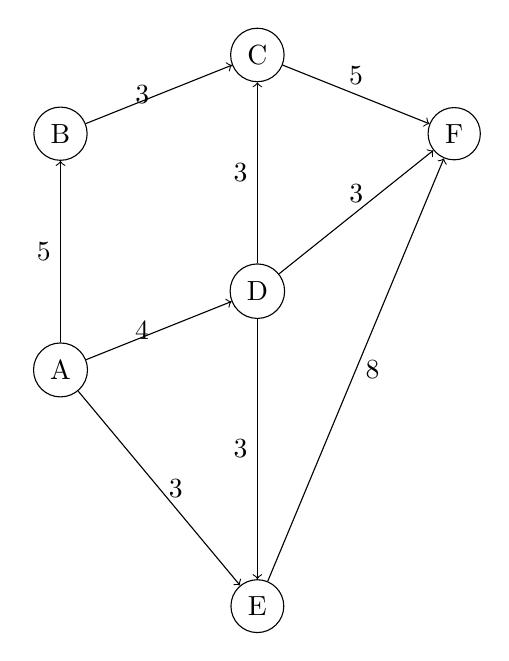
\begin{tikzpicture}

% Vertices:
\node[shape=circle,draw=black] (A) at (0,0)    {A};
\node[shape=circle,draw=black] (B) at (0,3)    {B};
\node[shape=circle,draw=black] (C) at (2.5,4)  {C};
\node[shape=circle,draw=black] (D) at (2.5,1)  {D};
\node[shape=circle,draw=black] (E) at (2.5,-3) {E};
\node[shape=circle,draw=black] (F) at (5,3)    {F};

% Edges:
\path [->](A) edge node[left]  {$5$} (B);
\path [->](B) edge node[left]  {$3$} (C);
\path [->](A) edge node[left]  {$4$} (D);
\path [->](D) edge node[left]  {$3$} (C);
\path [->](A) edge node[right] {$3$} (E);
\path [->](D) edge node[left]  {$3$} (E);
\path [->](D) edge node[above] {$3$} (F);
\path [->](C) edge node[above] {$5$} (F);
\path [->](E) edge node[right] {$8$} (F);   

\end{tikzpicture}


\begin{tikzpicture}

\begin{scope}[every node/.style={circle,thick,draw}]
  \node (A) at (0,0) {A};
  \node (B) at (0,3) {B};
  \node (C) at (2.5,4) {C};
  \node (D) at (2.5,1) {D};
  \node (E) at (2.5,-3) {E};
  \node (F) at (5,3) {F} ;
\end{scope}

\begin{scope}[>={Stealth[black]},
              every node/.style={fill=white,circle},
              every edge/.style={draw=red,very thick}]
  \path [->] (A) edge node {$5$} (B);
  \path [->] (B) edge node {$3$} (C);
  \path [->] (A) edge node {$4$} (D);
  \path [->] (D) edge node {$3$} (C);
  \path [->] (A) edge node {$3$} (E);
  \path [->] (D) edge node {$3$} (E);
  \path [->] (D) edge node {$3$} (F);
  \path [->] (C) edge node {$5$} (F);
  \path [->] (E) edge node {$8$} (F); 
  \path [->] (B) edge[bend right=60] node {$1$} (E); 
\end{scope}

\end{tikzpicture}
